\section{Case Study: Gossip Server}

A practical example is often useful to gain a better understanding of a process requiring different actors and multiple steps. The simple \textit{Gossip Application}, which can be found on GitHub (\url{https://github.com/patrickbucher/oauth2-demo}, with further information on how to run the applications and how to play with it), demonstrates the OAuth 2 authorization grant flow with three web applications written in Go:

\begin{description}
    \item The \textit{client}, which offers a web interface to retrieve gossip from a backend application. 
    \item The \textit{resource}, which offers a REST endpoint that provides gossip to authorized clients and users.
    \item The \textit{authserver}, which lets the client authorize itself to get access tokens, and validates access tokens for the resource before any gossip is delivered to the client.
\end{description}

The \textit{client} has a \texttt{client\_id} with a \texttt{client\_secret} (pre-shared between \textit{authserver} and \textit{client}), so that the \textit{client} can authenticate against the \textit{authserver}. The \textit{client} does not know the \textit{authserver}, it just knows how to authenticate towards \textit{any} authorization server: with its credentials, that is.

The \textit{resource owner} has its own gossip stored on the \textit{resource} server, and wants to access it through the \textit{client}. The \textit{resource owner} is neither aware of the \textit{resource server}, nor of the \textit{authserver}, but knows how to access the \textit{client}.

The \textit{resource} server knows the coordinates of the \textit{authserver}, and also knows that any request to its resources (the gossip) must be authorized using an access token, which must be verified against the \textit{authserver}.

\subsection{OAuth 2 Authorization Grant: A Conversation}

Even though the great Dijkstra frowned at antropomorphisms in computer science \cite{EWD936}, seeing the components of a system as human-like actors can often help gaining clarity. It is true that those actors do not «want» or «dismiss» anything on their own, it is the programmer's intention which is codified in those components. And the programmer needs to take different points of view when developing or understanding those components, and be aware of what components «knows» what and when.

A possible conversation between the actors of an OAuth 2 grant process -- the \textit{resource owner}, the \textit{client}, the \textit{authorisation server}, and the \textit{protected resource} -- might look as follows (the process can be followed along on \imgrefplain{fig:auth-grant}).

\begin{figure}
    \centering
    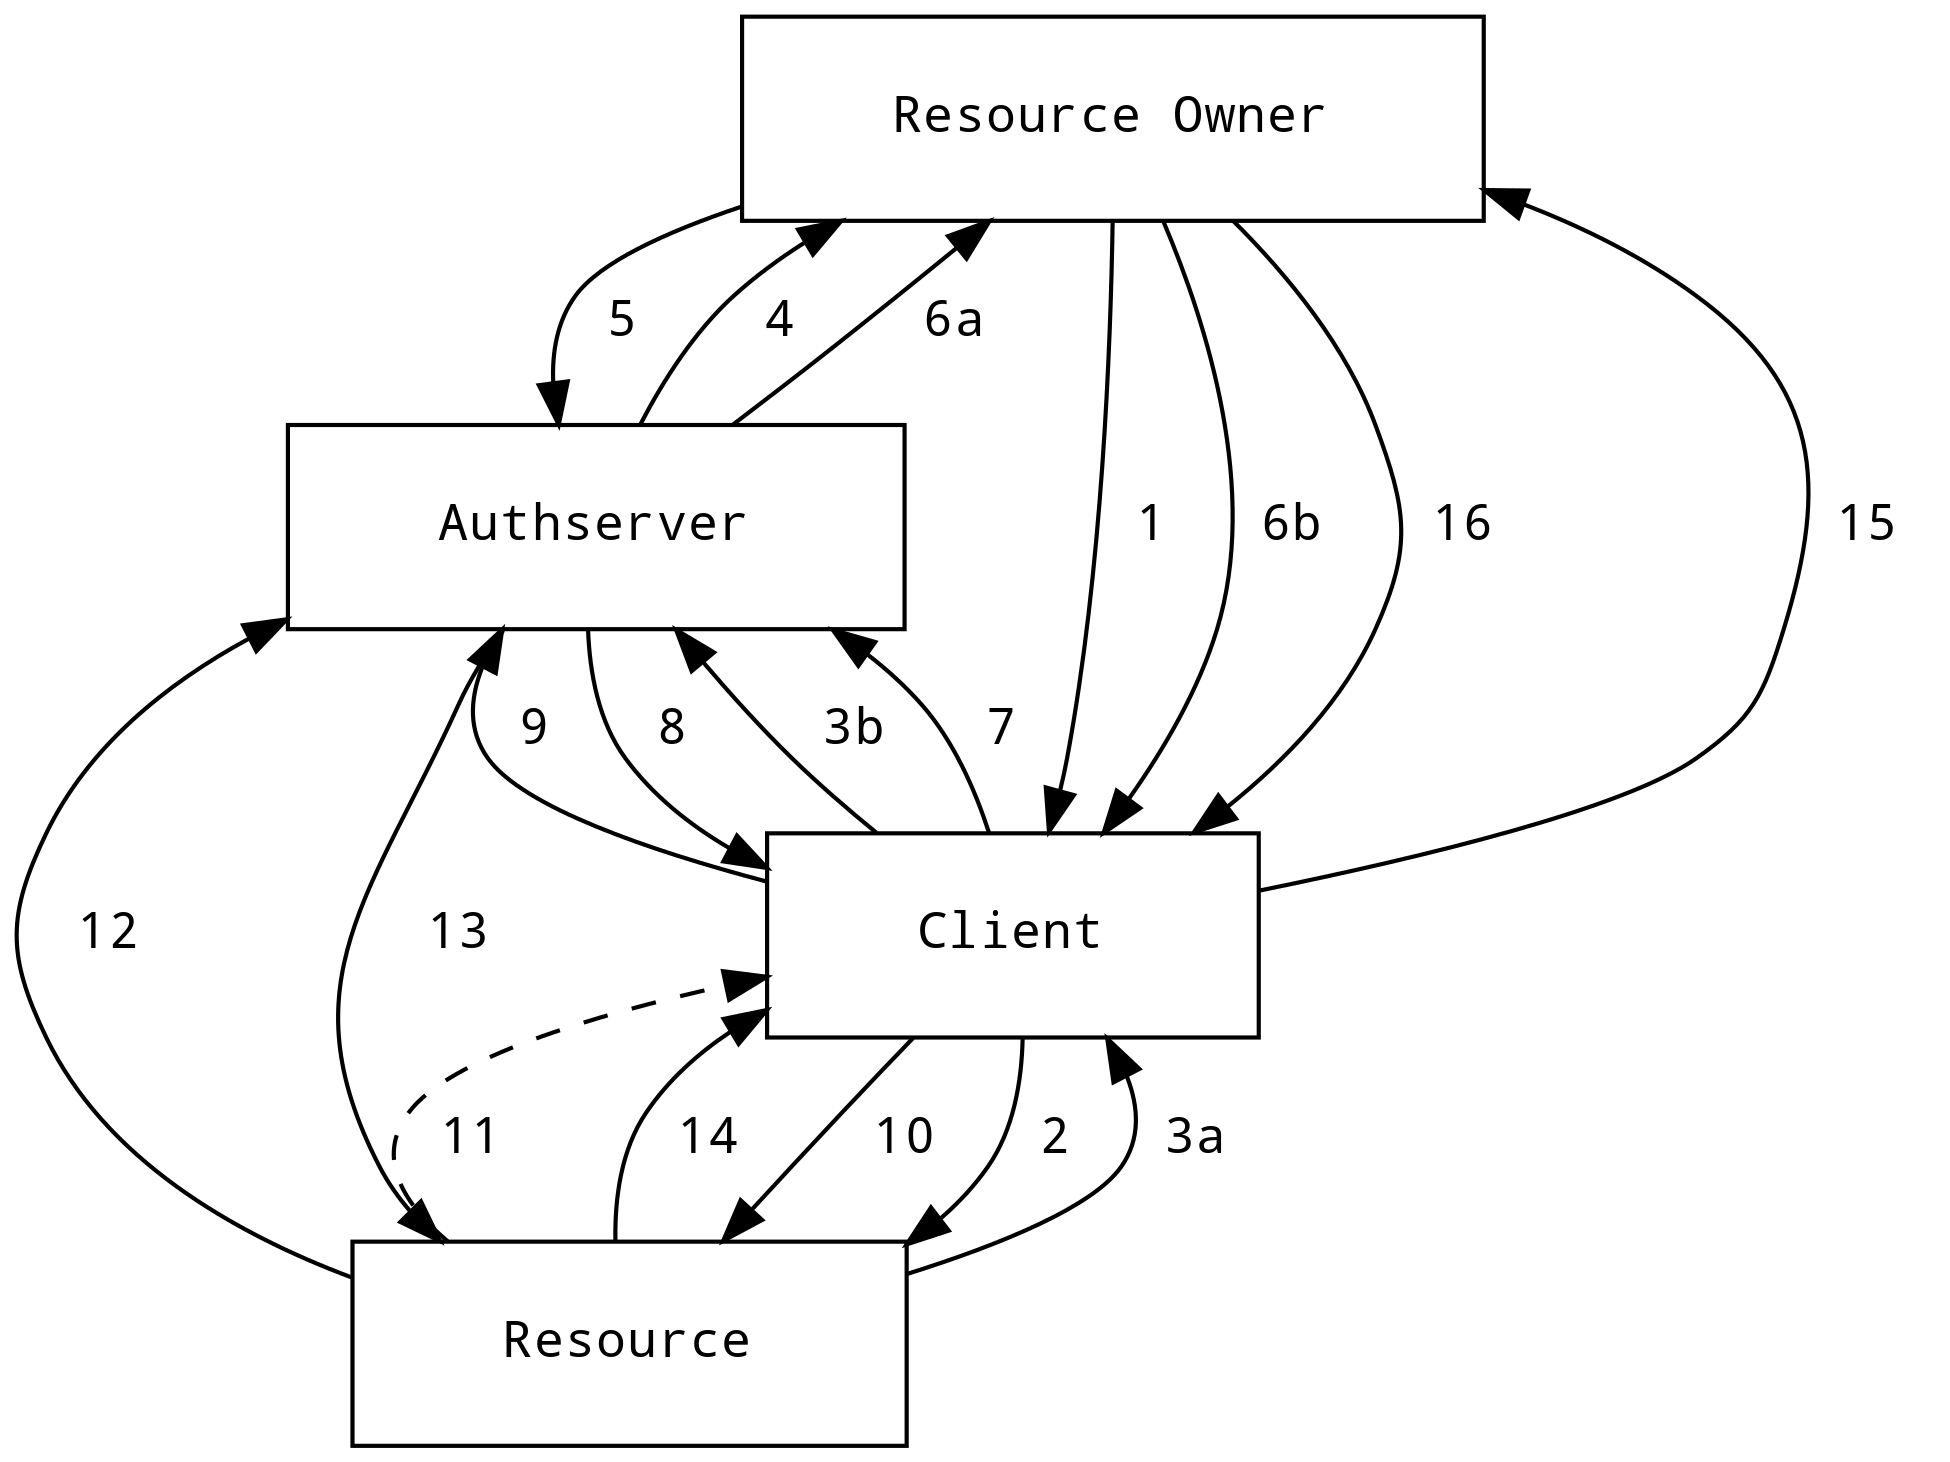
\includegraphics[width=\linewidth]{auth-grant.png}
    \caption{The OAuth 2 Authorization Grant}
    \label{fig:auth-grant}
\end{figure}

\subsubsection{Act I: Getting a Token}

In the first act, the protagonists are negotiating the access rights of a \textit{resource owner} delegated to the \textit{client}. The result of this process is the \texttt{access\_token}, which is an artifact representing the granted access right.

\begin{description}
    \item \texttt{1} \textbf{Resource Owner to Client} I have some gossip stored on the \textit{resource} server. Please retrieve that gossip for me, you can tell the \textit{resource} server that my name is «Joe».
    \item \texttt{2} \textbf{Client to Resource} Joe asked me to retrieve his gossip for him. Could you please hand me that over? I leave my coordinates, and a \texttt{state} identifier, just in case…
    \item \texttt{3a} \textbf{Resource to Client} Really? How can I be sure that it's really Joe asking for his gossip? If it really were Joe to ask me for the gossip, you'd bring along some \texttt{access\_token} to prove that Joe issued the request. Anybody could ask me to hand over Joe's gossip, but nobody but Joe has the rights to access it. I don't even know if you are trustworthy at all. You first must prove it! So here's the deal: Take this address, it belongs to the \textit{authserver}. I'm going to send it to Joe -- or whoever is using you at the moment… if somebody is actually using you! Joe has to identify himself with his username and password, and in the same step tell the \textit{authserver} that you are a trustworthy client. I'm writing down the coordinates of your \texttt{/callback} endpoint you told me about, so that the \textit{authserver} can come back to you after Joe authorized you, and I make sure the \textit{authserver} gets that note when I'm redirecting Joe to it. I'll also forward your \texttt{state} identifier, so you can remember this request later. OK, see you later… maybe.
    \item \texttt{3b} \textbf{Client} OK, let me… Wow! What is happening? The resource owner is getting forwarded away from me!
    \item \texttt{4} \textbf{Authserver to Resource Owner} Hi there, I'm the \textit{authserver}. Remember me? You probably registered here and even verified your email address some time ago. The protected \textit{resource} sent you here, because some \textit{client} tried to access your resources on your behalf. I don't know if that's fine for you. If you really requested the \textit{client} to get the protected resource for you, then please tell me your username and password. When you do that, you automatically authorize the \textit{client} to get your resources.
    \item \texttt{5} \textbf{Resource Owner to Authserver} Hey, of course I remember you. I use you now and then to login to web sites that trust you. So my username is «Joe» and my password is… \textit{[unintelligible]}. It really was me who asked the \textit{client} to fetch the resource for me, so you can trust it.
    \item \texttt{6a} \textbf{Authserver to Resource Owner} Hey Joe, I found your account, and the password you entered matches what is stored in my credentials store. I'm writing down that you trust the \textit{client} from now on. The \textit{resource} (we trust each other) gave me a note on how to send you back to the client, which I'm going to do now. Here's also an \texttt{auth\_code} the \textit{client} can use once to get an \texttt{access\_token} for you. Goodbye Joe! See you again once your token is expired!
    \item \texttt{6b} \textbf{Resource Owner} OK, it looks like there's a forward going on again…
    \item \texttt{7} \textbf{Client to Authserver} Wow, I just got called back from you! The \textit{resource} told me that this is going to happen! Glad to hear that Joe trusts me. (It's not that much of a surprise, actually, because he told me already that I should fetch his resource.) And I remember that \texttt{state} identifier, it belongs to the initial request Joe let me do. Thanks also for your coordinates and the \texttt{auth\_code}. I'm going to use them right away to fetch an \texttt{access\_token} from you. By the way: We already know each other. I once registered with my \texttt{client\_id}, and you gave me this \texttt{client\_secret} you hopefully still remember! Let me send those to you base64 encoded as a HTTP basic \texttt{Authorization} header. OK, can I please get an \texttt{access\_token} for Joe?
    \item \texttt{8} \textbf{Authserver to Client} Hello again, thanks for calling my \texttt{/token} endpoint. Let's see… Indeed, I remember the \texttt{client\_id} and \texttt{client\_secret} you sent to me, all so nicely and securely wrapped up in the \texttt{Authorization} header. And this is really the \texttt{auth\_code} I just sent you before. And it belongs to Joe. And Joe authorized you as a client. The \texttt{auth\_code} is a one-time password, so let's forget about it once you got the \texttt{access\_\-token}, all right? So here's your \texttt{access\_token}, I'm going to remember it. Now hurry up, this token is going to expire soon! And we don't want Joe to go through all this hassle again, do we?
    \item 9 \textbf{Client to Authserver} Great, thanks! I'm going to replay Joe's initial request right away, but this time I'll attach that token you've given me to the \textit{resource} in the \texttt{Authorization} header. See you later, maybe…
\end{description}

\subsubsection{Act II: Using a Token}

Once an \texttt{access\_token} is granted, it can be used to retrieve resources. The second act can be replayed many times, as long as the \texttt{access\_token} is valid.

\begin{description}
    \item \texttt{10} \textbf{Client to Resource} So, here's Joe's initial request again, but this time, I also got this nice \texttt{access\_token} with me. So open up and hand me over Joe's gossip! (He really is on a mission and wants to spread it…)
    \item \texttt{11} \textbf{Resource to Client} OK, now this is an \texttt{access\_token}? I don't know, but the \textit{authserver} does! Hang on, I quickly double check, if that is valid.
    \item \texttt{12} \textbf{Resource to Authserver} Hey, it's me, I've just redirected some \textit{client} to you a couple of seconds ago. I remember that he wanted to get Joe's resources. He gave me this \texttt{access\_token}. Is that thing valid?
    \item \texttt{13} \textbf{Authserver to Resource} Hello, my dear old friend! Let's see: Indeed, I issued such an \texttt{access\_\-token}, and it was only seconds ago. So the token is still valid. And I remember that I issued it for Joe's scope. Perfectly fine with me, go ahead and hand over Joe's resource to that \textit{client}!
    \item \texttt{14} \textbf{Resource to Client} Are you still there? OK, great! I have good news for you! The \texttt{access\_token} you sent to me is valid! So here's Joe's gossip! You can come back later to me. I'll always check that token against the \textit{authserver}, because only he knows all the security details. (I just know some gossip.)
    \item \texttt{15} \textbf{Client to Resource Owner} Hey Joe, here I am again! And I got your gossip with me. I'm going to display it as a HTML page. When you access it anytime soon, you're not required to authenticate yourself and authorize me again, because me, the \textit{authserver}, and the \textit{resource} managed to sort that out for you. But if you wait for too long, we might need to go through that whole process again. I'm so happy that we are all compiled programs that do just execute and not think too much…
    \item \texttt{16} \textbf{Resource Owner to Client} Hey, thanks for all that work! I'm now going to enjoy my gossip. See you later!
\end{description}
